
% Describe the performed solution with all possible details. Define necessary parameters, inputs, outputs and context of use, possible problems and when they can be applied. 

% Remember to define necessary concepts before using them, building the text from easiest definitions (not depending on previous definitions) to complex definitions (depending on previous definitions).

% E.g: 
% \begin{itemize}
%	\item Lost Communication: a lost communication occurs when the conditions of the environment are not sufficient or the distance between sender and receiver is to hight to transmit information.
%	\item Wait until rescue: when the robot loses its communication, the pre-designed state machine will stop the motors to keep the actual position. Energy safe mode will be enabled, at the same time that a channel transceiver daemon will send SOS messages every T and wait for reply during T sec. 
%\end{itemize}
% A communication efficient task scheduling system is designed to help multiple robots handle various task. 
% This system schedule task according to system resources, including system environment information, robot status and task specifications. Once this information is attained, the task scheduling system sends robot a set of task.

% \begin{itemize}
% 	\item \textbf{Robot.} Each robot is responsible for moving in 2-dimensional physical space as well as gathering measurement result from sensors. It has a rechargeable battery, and its level drops as robot moves and rotates.
% 	\item \textbf{Tasks.} Each task requires one or more robots to traverse a path in the workspace and carry out certain activitys\cite{Ivan2017}.
% 	\item \textbf{Environment.} In this project, all robots are considered moving in an office environment that contains a corridor along the central x-axis and 16 rooms located around the corridor. The environment factors, such as room locations and occupation possibilities help task scheduling.
% \end{itemize}
\chapter{Approach}

\section{Architecture Design}
\label{sec:architecture_design}

The architecture of the system consists of several parts: centralized pool, robot controller, navigation stack, charging station, and system environment(Figure \ref{fig:system_architecture}). 

\begin{itemize}
 \item \textbf{Centralized Pool.} The centralized pool is the global controller that receives information about the robots and the environment and make decisions base on the information. To be more precise, the centralized pool uses this information in two ways. It schedules the robot's navigation tasks according to the information and can also assign robots to explore the room lacking information. It consists of several modules: multi-robot task scheduling module, map information, database, execution, and monitoring. The database stores dynamic indoor environment information such as room occupation data. The map information modules contain the static map information(Figure \ref{fig:database_er}). The execution and monitoring module interacts with robots. The multi-robot task scheduling module selects tasks in the database based on the robot and environment information and then give the task to the execution and monitoring module.

 \item \textbf{Robot Controller.} A robot controller contains several modules: local task queue, execution, and robot activity. The local task queue stores tasks that the robot needs to complete sequentially. The execution module receives commands from the centralized pool and decides when and which task the robot should run. The robot activity module performs tasks in the local task queue when it receives the execution module's decision. The robot activity module also interacts with the office environment and ROS navigation stack. 

 \item \textbf{Navigation stack.} The move\_base node provides a ROS interface for configuring, running, and interacting with the navigation stack on a robot. It makes the robot move to desired positions using the navigation stack. Its advantages include optionally performing recovery behaviors when the robot is stuck:

Obstacles outside the area specified by the user on the map will be removed.
If possible, the robot will rotate to clear the space.
If this fails, the robot will clear its map more aggressively, removing all obstacles outside the rectangular area so that the robot can rotate in place within the rectangle.
If all this fails, the robot will consider its goal unreachable and print the abort details to ROS\cite{MOVEBASE}.
\end{itemize} 

\begin{figure}[htbp]
 \centering
 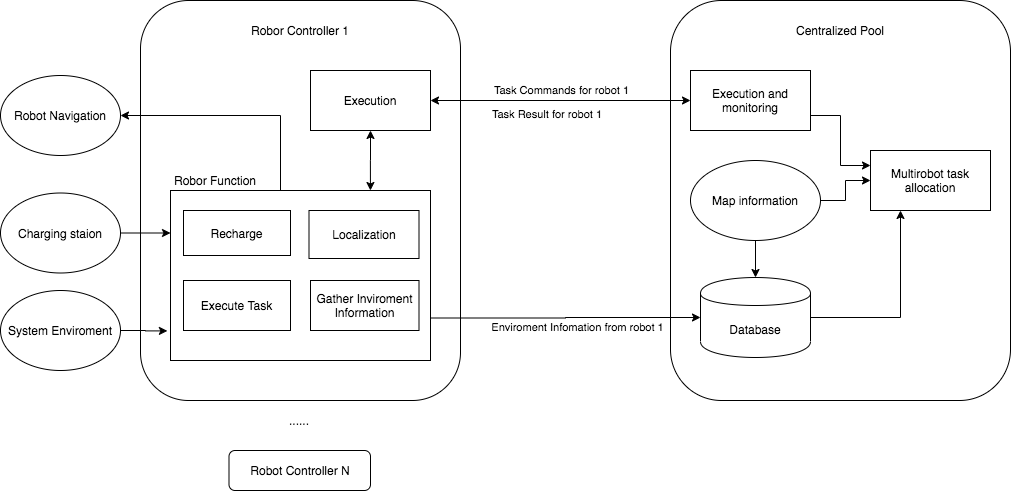
\includegraphics[width = 0.9\textwidth]{content/images/ch3/architecture.drawio.png}
 \caption{Multi-robot Task Scheduling Architecture.}
 \label{fig:system_architecture}
\end{figure}

\section{Gather Information Approach}
\label{sec:environment_and_gather_information_approach}

%\subsection{Gather Infomation Approach}
This project aims to schedule tasks for robots based on the room occupation information gathered about room occupation. Room occupation means the probability of someone in the office. In other words, in a typical office environment, people have different working schedules. If at least one person is in the office, the office is considered occupied. The first is to equip the robot with sensors and tools. For example, robotic tools such as Laser Distance Sensor (LDS) Camera and infrared sensor module can detect obstacles include doors. 
 However, compared with the entire office environment, the robot's perspective is limited, and the field within the sensing range is relatively narrow. Therefore, the use of external environment information sources is essential to bridge the local knowledge gap. The second is to establish a distributed IoT network. But gateways connect sensors, and gateways need to connect to the Internet. They consume much energy. The third method is to install wireless sensors on the doors. The wireless communications include Bluetooth Low Energy (BLE) \cite{BLEWeb}, ZigBee \cite{ZigBeeWeb}, ANT \cite{ANTWeb} , etc. This experiment uses the third method. A wireless module called SensorTag was used because it has a long battery life and has multiple sensors. The acceleration sensor can be used to infer the opening and closing of the door. An open door means someone in the room, and the room is occupied. A closed-door means that there is no one in the room and the room is not occupied. 

Robots interact with sensors while navigating in the office environment and report this environment information to the centralized pool. The centralized pool is the global controller that receives room occupation information about the robots and the environment and make decisions base on the information.  The way centralized pool storing and making decisions base on the information is discussed in section \ref{sec:task_scheduling_procedure}.

\section{Task Composition and Decomposition Approach}
\label{sec:task_explan}

\subsection{Task Specification}

The overall system goal is to gather room occupation information for a long time continuously, and the centralized pool assigns tasks for robots based on the robot and environmental information. The centralized pool is the global controller that receives information about the robots and the environment and make decisions base on the information \ref{sec:architecture_design}. 

Task information consists of the following parts: The Task ID is a unique task identification. The task name is a description of the main activity.
Three task names are defined: ``gather information task'' asks a robot to gathers environment information from sensors, ``navigation task'' asks a robot to move to a point, and ``charging task'' asks the robot to refill its battery at charging stations. The start time refers to when the robot should move towards the target. A starting time is given when the task is created. This time can be a time in the future or empty (no time limit). The finish time refers to when the robot finishes the task. Targets include doors, points, and charging stations. Target ID is unique target identification. Robot ID is a unique robot identification. Task Priority describes the importance of the task. Once a task failed, its priority will be increased by one and reused in task scheduling. If this task has already the highest priority, the task fails. Task status are ``Created'', ``Succeeded'', ``Failed'', ``To rerun'', ``Error''. The difference between task status is discussed in Figure \ref{fig:centralized_task_handle}. Task dependency means the required last task. If task B has a dependency of task A, task A needs to be preceded by tasks B. Those dependent tasks should be composed in the centralized pool. The Task description is one sentence. The description of a succeeded task is ``succeeded''. The description of a failed task is its failure reason. A example of  task specifications are stored in ``task table'' in database (Table \ref{tab:db_task_table}).





\subsection{Task Composition and Decomposition}
Tasks can be distinguished into ``simple tasks'' and ``Complex tasks''. ``Simple tasks'' comprises a single target position that can be performed by a single robot. A ``Complex tasks'' can be broken up or decomposed into multiple ``small tasks''. Those sub-tasks of a complex task need to be performed by the same robot. A ``complex task'' can have only one sub-tasks.
In this project, the centralized poll not only can create ``simple tasks'' according to task specifications (Table \ref{tab:db_task_table}) but also can analyze the dependencies of ``simple tasks'' and form a dependency chain to compose ``complex tasks''. The robot (robot controller) can decompose a ``Complex task'' to ``simple tasks'' and execute ``small tasks'' according to their dependencies.

\section{Multi-robot Task Scheduling Approach}
\label{sec:task_scheduling_approach}

The multi-robot task scheduling module in the architecture should perform multi-robot task scheduling. 
The implementation of task scheduling is shown in Chapter \ref{sec:task_scheduling_procedure}. There are some general rules for multi-robot task scheduling.


\begin{enumerate}
 \item When the robot's energy below 10\%, the centralized pool's task scheduling module (Chapter \ref{sec:architecture_design}) creates and sends a ``charging task''  to the robot based on rule discribed in in Chapter \ref{sec:create_charging_task}.

 \item When the robot's energy above 10\% and there are ``navigation tasks'' in the database, the task module composes simple tasks into complex tasks and selects a complex task for the robot according to the rule shown in Chapter \ref{sec:select_navigation_task}.

 \item  When the robot's energy above 10\% and there is no ``navigation task'' or the cost of all navigation tasks is higher than the threshold, create a ``gather information task'' for the robot according to the rule discussed in Chapter  \ref{sec:create_gather_information_task}.
\end{enumerate}

\subsection{Select Navigation Task}
\label{sec:select_navigation_task}
When one of the ``complex navigation tasks'' should be selected for robot, In order to select an ``navigation task'', the decision variables are considered. 
\paragraph{Decision variables used to select navigation tasks.}
\begin{itemize}
\item \textbf{Task Priority.} The priority is discussed Chapter \ref{sec:task_table}.
\item \textbf{Product of Door Open Possibility.} The product of open possibilities of doors on trajectory: All doors that the robot will pass through when moving from its location to the target point.
 An example of ``measurement result'' table is shown in Table \ref{tab:db_measurement_result}, an example of ``open probability'' table is shown in Table \ref{tab:db_open_possibilities}. 
\item \textbf{Waiting Time. } The waiting time is the difference between the current simulation time and start time of the first task to be executed. $T_{waiting} = T_{first\_task} - T_{now}$
\item \textbf{Battery Consumption.} The Battery Consumption is related to robot trajectory. For a Large ``navigation task'' that contains n simple task, Equation \ref{eq:battery_consumption} can be used to calculate battery consumption. The centralized pool will send the task with the lowest cost to this robot.
\end{itemize}

Equation \ref{eq:large_execute_task_cost} are used to calculate the cost. The ``complex navigation tasks'' with the lowest cost will be selected.

\begin{equation}
 \label{eq:large_execute_task_cost} 
 \begin{aligned}
 & \mbox{W: Weight } \\
 & \mbox{n: Number of doors} \\
 & \mbox{Cost}_{\mbox{Large navigation task}} = \frac{W_{\mbox{battery}} \times \mbox{Battery consumtion}}{n} + W_{\mbox{waiting}} \times \mbox{waiting time} \\
 & + W_{\mbox{probability}} \times \prod\limits_{i=1}^n \mbox{Door open probability} + W_{\mbox{priority}} \times \mbox{Priority}
 \end{aligned}
\end{equation}




\begin{equation}
\begin{aligned}
\label{eq:battery_consumption}
& \mbox{B:Battery consumption } \\
& \mbox{W: Weight } \\
& \mbox{m: Number of waypoint } \\
& \mbox{n: Number of simple task} \\
& B_{\mbox{complex task}} = \sum_{\mbox{task}_1}^{\mbox{task}_n} B_{\mbox{trajectory}} \\
& = \sum_{t = \mbox{task}_1}^{\mbox{task}_n} \sum_{\mbox{waypoint}_1}^{\mbox{waypoint}_m} [W_{\mbox{position}} \times \mbox{position variation}+W_{\mbox{angle}} \times \mbox{angle variation}]\\
& = \sum_{t = \mbox{task}_1}^{\mbox{task}_n} \sum_{p = \mbox{waypoint}_1}^{\mbox{waypoint}_m} [ W_{\mbox{position}} \times \sqrt{(x_p-x_{p-1} )^2+(y_p-y_{p-1} )^2} \\
& + W_{\mbox{angle}} \times 2 \times \arccos(w_p)] 
\end{aligned}
\end{equation}


\subsection{Create Gather Information Task}
\label{sec:create_gather_information_task}
Robot can perform ``gather environment information task'' to gather more measurement results and furthermore improve the accuracy of ``open possibilities'' table.
To create a ``gather environment information task'', Equation \ref{eq:door_cost} and following decision variables are used to calculate the costs of doors. A ``gather environment information task'' to the door with the lowest cost will be created.
\paragraph{Decision variables used to create a gather information task}
\begin{itemize}
 \item \textbf{Door Last Update Time.} The latest timestamp when the door is measured.
 \item \textbf{Product of Door Open Possibility.} The product of open possibilities of doors on trajectory: All doors that the robot will pass through when moving from its location to the front of the target door.
 \item \textbf{Battery Consumption.} The battery consumption is related to the trajectory from the robot to the front of the door. Equation \ref{eq:battery_consumption} can be used to calculate battery consumption.
\end{itemize}

\begin{equation}
 \label{eq:door_cost}
 \begin{aligned}
 & \mbox{W: Weight } \\
 & \mbox{n: Number of doors on trajectory} \\ 
 & \mbox{Cost}_{\mbox{door}} = \frac{W_{\mbox{battery}} \times \mbox{Battery consumtion}}{n} + W_{\mbox{time}} \times (T_{\mbox{last update}} - T_{\mbox{now}}) \\
 & + W_{\mbox{probability}} \times \prod\limits_{i=1}^n \mbox{Door open probability}
 \end{aligned}
\end{equation}





\subsection{Create Charging Task}
\label{sec:create_charging_task}
Once a robot sends task requests to the centralized pool, the centralized pool should determine whether this robot needs charging. If yes, it should create a ``charging task'' for the robot. 
To create a ``charging task'', Equation \ref{eq:door_cost} and following decision variables are used to calculate the costs of charging station. A ``charging task'' to the charging station with the lowest cost will be created.


\paragraph{Decision variables used to create a charging task.}
\begin{itemize}
 \item \textbf{Remain Time.} It describes how long will a charging station be free. 
 \item \textbf{Battery Consumption.} Similar to ``navigation task'' scheduling, the battery consumption is related to the trajectory from robot to the charging station. Equation \ref{eq:battery_consumption} can be used to calculate battery consumption.
\end{itemize}

\begin{equation} 
\label{eq:charging_station_cost}
\begin{aligned}
 & \mbox{W: Weight } \\
 & \mbox{Cost}_{\mbox{charging station}} = \frac{W_{\mbox{battery}} \times \mbox{battery consumtion}}{n} + W_{\mbox{time}} \times T_{\mbox{remain}}
\end{aligned}
\end{equation}

